In dem folgenden Kapitel sollen die Ergebnisse der Implementierungen ausgewertet und analysiert werden. Dafür werden einige ausgewählte Kriterien anhand der Implementierungen wund weiteren Quellen analysiert und verglichen.

\section{Performance und Entwicklung}
Ein wichtiger Faktor für die Entwicklung einer Applikation ist die Performance und die Entwicklung. Dabei ist die Performance ein wichtiger Faktor, der die Erfahrung bei der Benutzung beeinflusst. Daher sollten Apps möglichst performant laufen, um die Ressourcen des Gerätes zu schonen und einen flüssigen Ablauf zu ermöglichen. Außerdem benötigen Entwickler einen einfachen und zeitsparenden Ablauf für typische Entwicklungsoperationen, wie etwa das anfängliche Kompilieren, oder das Laden von Änderungen. Auch die Möglichkeiten des Debuggen und Testen spielen bei der Entwicklung eine Rolle. Diese Faktoren sollen im Folgenden analysiert werden.

\subsubsection{Performance}

\begin{table}[ht]
\centering
\caption{Performancemessung der verschiedenen Applikationen}
\begin{tabular}{ |p{4cm}||p{3cm}|p{2cm}|p{2cm}|p{2cm}|p{2cm}| }
 \hline
 Parameter & Flutter-Hybrid & Flutter & Kotlin-Nativ & Kotlin-WebView \\
 \hline
 Durchschnittliche CPU-Auslastung       &   2,54\%&   1,96\%& 0,9\%& 1,8\%\\
  \hline
 Maximale CPU- Auslastung  & 9,8\%& 6,4\%& 3,6\%& 7,4\%\\
  \hline
 Durchschnittliche RAM-Auslastung & 215,38 MB& 150,68MB& 86,74MB& 107,68MB\\
  \hline
 Maximale RAM- Auslastung & 238,00MB& 175,46MB& 100,64MB& 117,06MB\\
  \hline
 App-Größe & 7,4MB& 7,2MB& 5,2MB& 4,4MB\\
  \hline
 Maximale Startzeit & 532ms& 452ms& 263ms& 486ms\\
 \hline
 Durchschnittliche Renderzeit &8,68ms& 5,12ms& 9,04ms& 21,88ms\\
 \hline
\end{tabular}
\label{tab:evaluations_performance}
\end{table}

In Tabelle \ref{tab:evaluations_performance} sind die Ergebnisse der Performance-Messungen zu sehen, die an den in Kapitel \ref{cha:4_Entwicklung} beschriebenen Implementierungen durchgeführt wurden. Dabei wurden die Durchscnittliche und maximale Auslastung der CPU und des RAMs, sowie die App-Größe, Maximale Startzeit der Applikation und durchschnittliche Renderzeit gemessen. 
Die Renderzeit entspricht dabei der Zeit, die benötigt wird, bis eine Änderungen der Benutzeroberfläche fertig verarbeitet und die Änderungen angezeigt werden kann.

Die Messungen wurden mit dem Programm Apptim\footnote{https://www.apptim.com/} durchgeführt. Dieses zeichnet die Performance von Applikationen während der Nutzung auf einem verbundenen Gerät auf. Die Tests wurden auf einem Google Pixel 5 durchgeführt das mit Android 12 beziehungsweise API Level 31 läuft. Es hat dabei 8GB DDR4-RAM und eine 8-Kern-CPU, die mit durchschnittlich 1,9 GHz getaktet ist.
Der Test wurde dabei für jede Implementierung 5 mal wiederholt und am Ende aus den Ergebnissen ein Durchschnittswert gebildet.
Die Apps wurden nach jeder Nutzung zurückgesetzt und alle anderen Applikationen wurden während der Tests beendet.
Außerdem wurde jeweils die Release-Version der Applikationen installiert, so dass die Performance gemessen wird, die auch ein Nutzer so messen könnte.

Hierbei ist erkennbar, dass die native Implementierung insgesamt die performanteste ist und dabei gerade einmal etwa die Hälfte der Auslastung erreicht wie die Flutter Applikation.
Hingegen hat die hybride Flutter App im Vergleich die höchste Auslastung und Startzeit.
Auf die Programmiersprachen betrachtet, haben die mit Dart programmierten Flutter Applikationen die geringste Renderzeit, während die Auslastung des RAMs bei den Android Applikationen deutlich geringer ist.
Die Implementierungen mit einem WebContainer, also die hybride und cross-kompilierte hybride, verschlechtern sich, im Vergleich zu den anderen beiden Implementierungen, in der Performance deutlich. Das lässt darauf schließen, dass ein Web-Container eine  Performanceverschlechterung bedeutet. So ist etwa die hybride Applikation in den Messwerten ähnlich zu der cross-kompilierten Applikation, obwohl sie lediglich einen Web-Container ausführt und anzeigt, während die Flutter App die komplette Benutzeroberfläche und Kommunikation mit dem Server ausführt. Dies ist auch in der deutlich geringeren App-Größe der WebView-Applikation zu erkennen.  

Die geringere Renderzeit der Flutter Applikationen ist insofern unerwartet, da Flutter die Applikation in nativen Code übersetzt und somit eine ähnliche bis schlechtere Leistung erwartet werden würde. Jedoch nutzt Flutter für die UI keinen nativen Code, sondern eine eigene Grafikbibliothek namens Skia\footnote{https://skia.org/}. Mit Hilfe von Skia sind Flutter Apps von der Renderpipeline des nativen Systems unabhängig und erreichen dadurch eine kürzere Renderzeit \cite{Thiele_2018}. Dabei wird bei Flutter die einzelnen Elemente der Benutzeroberfläche auf eine Art Leinwand gemalt. Die Oberfläche wirkt dabei jedoch nativ für die Plattformen Android und iOS, da je nach Plattform unterschiedliche Designgrundlagen verwendet werden, um die UI zu erstellen\cite{jose_flutter}.

Biorn Hansen et al\cite{BirnHansen.2020} sagen in ihrer Auswertung, dass sie einen deutlichen Verschlechterung der Performance von Flutter bei der Nutzung einer Datenbank feststellen konnten. Deshalb wurde sowohl die Flutter App als auch die native Android App  jeweils mit und ohne einer Datenbank gemessen und der Unterschied zwischen den zwei Messungen berechnet. Das Ergebnis ist dabei in Tabelle \ref{tab:evaluations_performance_Overhead_database} zu sehen.

\begin{table}[ht]
\centering
\caption{Unterschied bei Implementierung mit zusätzlicher Datenbankimplementierung}
\begin{tabular}{ |p{7cm}||wc{3.5cm}|wc{3.5cm}|}
 \hline
 Parameter & Flutter &  Kotlin-Nativ \\
 \hline
 Durchschnittliche CPU-Auslastung       &  0,44\%&   0,26\%\\
  \hline
 Maximale CPU-Auslastung  & 2,2\%& 2,6\%\\
  \hline
 Durchschnittliche RAM-Auslastung & 5,64 MB& 18,04MB\\
  \hline
 Maximale RAM-Auslastung & 4,98MB& 39,64MB\\
  \hline
 App-Größe & 0,1MB& 0,1MB\\
  \hline
 Maximale Startzeit & 221ms& 162ms\\
 \hline
 Durchschnittliche Renderzeit &0,82ms& 4,68ms\\
 \hline
\end{tabular}
\label{tab:evaluations_performance_Overhead_database}
\end{table}

Die Ergebnisse zeigen einen Anstieg der RAM Auslastung, der bei der nativen Implementierung etwa drei mal so hoch ist, wie bei der Flutter implementierung. Dafür ist die Startzeit und durchschnittliche CPU Auslastung bei der Flutter Implementierung mehr erhöht als bei der Nativen. In Bezug auf Tabelle \ref{tab:evaluations_performance} und ihrer Auswertung nehmen, lässt sich jedoch sagen, dass kein deutlicher Unterschied in der Auswirkung auf die Performance der Applikation zu erkennen ist.

Für den Aspekt der Performance kann insgesamt festgestellt werden, dass die native Implementierung außer in der Renderzeit am besten war. Flutter kann durch die schnelle Renderzeit überzeugen und ist auch insgesamt für den Nutzer nicht spürbar langsamer, da die Unterschiede im Millisekunden- beziehungsweise im Einstelligen Prozentebereich liegen. Die Nutzung einer WebView wie sie die hybride Flutter App und die hybride App benutzen hat sich außerdem als negativen Faktor für die Performance dargestellt.
Insgesamt lässt dies den Schluss zu, dass bei einer hohen Dringlichkeit der Performance eine native Entwicklung ratsam ist, jedoch eine cross-kompilierte Flutter-Implementierung ebenfalls möglich ist.

\subsubsection{Dauer typischer Entwicklungsoperationen}
Wenn es um Entwicklungszeit und Fortschritt in der Entwicklung geht, dann ist ein großer Faktor, wie lange die App braucht um gebaut zu werden und wie lange es dauert um Änderungen in der App anzuzeigen. Oft muss bei der Entwicklung von Oberflächen einige Kleinigkeiten geändert und dann überprüft werden, ob die Änderung den gewünschten Effekt hatte. Deshalb sind vor allem kurze Ladezeiten von Änderungen besonders wichtig.

Die genauen Zahlen sind immer von der genutzten Hardware und der Projektgröße abhängig, sie können aber gut genutzt werden um den Unterschied zu vergleichen. 
Für diese Arbeit wurden die Tests wieder fünf mal wiederholt und am Ende ein Durchschnitt gebildet. Als Hardware wurde ein PC mit 32GB RAM und einer Ryzen 5 2600 CPU genutzt. 
Die betrachteten Parameter sind dabei die Dauer des erstmaligen kompilieren, die Dauer eines Neubaus auf Basis eines bestehenden Caches, die Dauer bis Layoutänderungen und bis Anwendungslogik geladen wurde. Diese Tests für diese Werte wurden im Debug-Modus durchgeführt. Dieser ist der typische Modus während der Entwicklung , da er einige Einstellungen besitzt, die das Debuggen oder ähnliches ermöglichen. Neben diesen Parametern wurde außerdem noch die Kompilierzeit im Release Modus aufgezeichnet, um zu messen, wie lange es dauert eine Version zur Veröffentlichung zu bauen. Die Ergebnisse sind in Tabelle \ref{tab:evaluations_build_time} zu sehen.

\begin{table}
\centering
\caption{Dauer typischer Entwicklungsoperationen in Sekunden}
\begin{tabular}{ |p{4cm}||p{3cm}|p{2cm}|p{2cm}|p{3cm}|p{3cm}| }
 \hline
 Funktion & Flutter-Hybrid & Flutter & Kotlin-Nativ & Kotlin-WebView \\
 \hline
 Build Zeit Release       &   59,20&   54,22& 40,92& 22,42\\
  \hline
 Build Zeit Debug  & 33,78& 28,76& 20,20& 20,19\\
  \hline
 Erneuter Build mit Cache & 8,80& 8,36& 3,36& 3,21\\
  \hline
 Neuladen nach Layoutänderg & 0,59& 0,60& 2,59& 2,64\\
  \hline
 Neuladen nach Logikänderung & 0,626& 0,622& 3,183& 2,635\\
  \hline
\end{tabular}
\label{tab:evaluations_build_time}
\end{table}

Bei der Analyse der Daten fällt auf, dass die Zeit zum Bauen der Applikationen  bei Flutter Applikationen im Vergleich zu den mit Kotlin implementierten Ansätzen höher ist. 
Auch bei dem erneuten Bauen mit vorhandenen Build-Cache sind die Kotlin-Versionen etwa doppelt so schnell wie die Flutter Implementierungen.
Bis auf den hybriden Ansatz braucht die Erstellung der Release-Version etwa doppelt so lang wie der Debug-Version. 
Bei der hybriden Version ist hier kein großer Unterschied, was an der geringen Größe der Programmierung liegen dürfte.

Ein großer Unterschied ist jedoch die Neuladezeit nach einer Änderung im Quellcode. Denn Flutter ist dank des so genannten HotReload Features deutlich schneller und benötigt somit gerade einmal 1/5 der Zeit der Koltin Applikationen. Dazu kommt, dass beim Neuladen mit Kotlin, die Applikation vom Startbildschirm neu startet, während Flutter nur die Änderungen in die aktuelle Seite lädt und diese neu rendert. Dadurch muss nicht erst wieder zu der aktuell entwickelten Stelle zurückgekehrt werden. So wird etwa die Farbe eines Textes im Fluttercode geändert und innerhalb von 600ms angezeigt. So wird nicht nur Zeit gespart, sondern es kann sich auch besser darauf konzentriert werden, eine ordentliche Benutzeroberfläche zu entwickeln.

Ein Grund für die Geschwindigkeit der Flutter Applikation beim Laden von Änderung liegt in der Architektur von Flutter. So ist Flutter zwar im Release Modus eine cross-kompilierte Anwendung. Jedoch ist Flutter im Debug-Modus eine interpretierte Anwendung \cite{flutter_debug_dart}. So wird Dart in diesem Modus nicht im vorherein kompiliert sondern erst wenn der Code ausgeführt wird. So müssen die Änderungen nur an die entsprechende Stelle geladen werden und die aktuell angezeigte Seite neu gebaut werden. Dadurch sinkt jedoch die Performance der Applikation, da wie bei interpretierten Applikationen typisch, der Code vor jeder Ausführung compiliert werden muss. Dies ist jedoch im Debug Modus nicht schlimm, da es hier auf die Fähigkeit zur Entwicklung ankommt. Dart bietet noch einen dritten Modus an, in dem eine Applikation auf einem Gerät installiert werden kann, dem sogenannten Profile-Modus \footnote{https://docs.flutter.dev/testing/build-modes\#profile}\cite{flutter_debug_dart}. 
Dieser wird benötigt um eine Überprüfung der korrekten Funktionalität der kompilierten Version zu ermöglichen, dabei jedoch immer noch die Möglichkeit zu haben, den Code zu debuggen. Daher wird in diesem Modus die App bereits im vornherein kompiliert, jedoch noch keine Optmierungen am Code vorgenommen.

Wie festgestellt werden konnte, hat der Vergleich der Dauer typischer Entwicklungsoperationen weniger mit dem Ansatz als mit der gewählten Programmiersprache oder Framework zu tun. Dabei sind die mit Kotlin implementierten Anwendungen zwar schneller kompiliert, jedoch kann Flutter durch die intelligente Nutzung verschiedener Compiler für verschiedene Applikationsmodi bei dem Laden von Änderungen in die App überzeugen.

\subsubsection{Debuggen und Testen}
Bei Debuggen und Testen haben technisch gesehen alle Apps die gleichen Voraussetzungen. So unterstützen alle hier benutzten Programmiersprachen sowohl Konsolenausgaben und Breakpoints im Code. Auch Tests sind bei allen betrachteten Fällen implementierbar.

Allerdings unterscheiden sich die verschiedenen Ansätze im Aufwand. So muss bei dem hybriden und dem gemischten Ansatz die beiden Teile der Implementierung getrennt betrachtet werden, wenn die Web-Implementierung nicht innerhalb der Applikation, sonder auf einem externen Server läuft. Bei nativen Implementierungen entsteht ein erhöhter Aufwand, da Tests für jede einzelne programmierte Implementierung definiert werden müssen. Bei der cross-kompilierten Anwendung muss dies lediglich einmal getan werden, da alle unterschiedlichen Plattformen auf einer Codebasis aufbauen.

Auf den Cross-Plattform Ansätzen, also allen außer dem Nativen, lassen sich Implementierungsfehler einfacher reproduzieren, da diese auf allen unterstützten Geräten auftreten. Dies ist bei den nativen Applikationen nicht der Fall, da hier Fehler nur in einer Implementierung sein können.

Beim Faktor Debuggen und Testen kann also festgestellt werden, dass Implementierungen mit einem Fehler einen geringeren Aufwand und bessere Reproduzierbarkeit bedeuten. Jedoch ist sowohl das Testen und Debuggen bei allen Ansätzen Problemlos möglich, lediglich der Aufwand unterscheidet sich.

\section{Entwicklergemeinschaft}
Die Entwicklergemeinschaft ist ein weiterer Faktor für die Wahl einer Technologie. Denn wenn es keine Community gibt, wird es schwer Entwickler oder auch Lösungen für Probleme zu finden, ohne sie selber zu entwickeln. Dabei helfen neben Bibliotheken und Dokumentation auch die Zahl der aktiven Leute auf Frage und Antwort Plattformen wie Stackoverflow\footnote{https://stackoverflow.com/}.  Die genauen Zahlen derEntwickler beziehugnsweise der Populärität sind dabei nicht genau bestimmbar. Sie können jedoch anhand einiger Faktoren annähernd bestimmt beziehungsweise verglichen werden.

\subsubsection{Star-History}
Ein erster Anhaltspunkt ist die Anzahl der sogennatnen Stars auf den Github-Repositories der Programmiersprachen bzw. Frameworks. Es gibt an, wie viele Leute sich die Repositories mit einem Stern markiert haben, um über Neuerungen informiert zu werden. Es gibt also keine absolute Zahl wie viele Leute mit einem Framework oder Programmiersprache entwickeln, es zeigt jedoch ganz gut wie viel Interesse an der Entwicklung besteht.

\begin{figure}[ht]
  \centering
  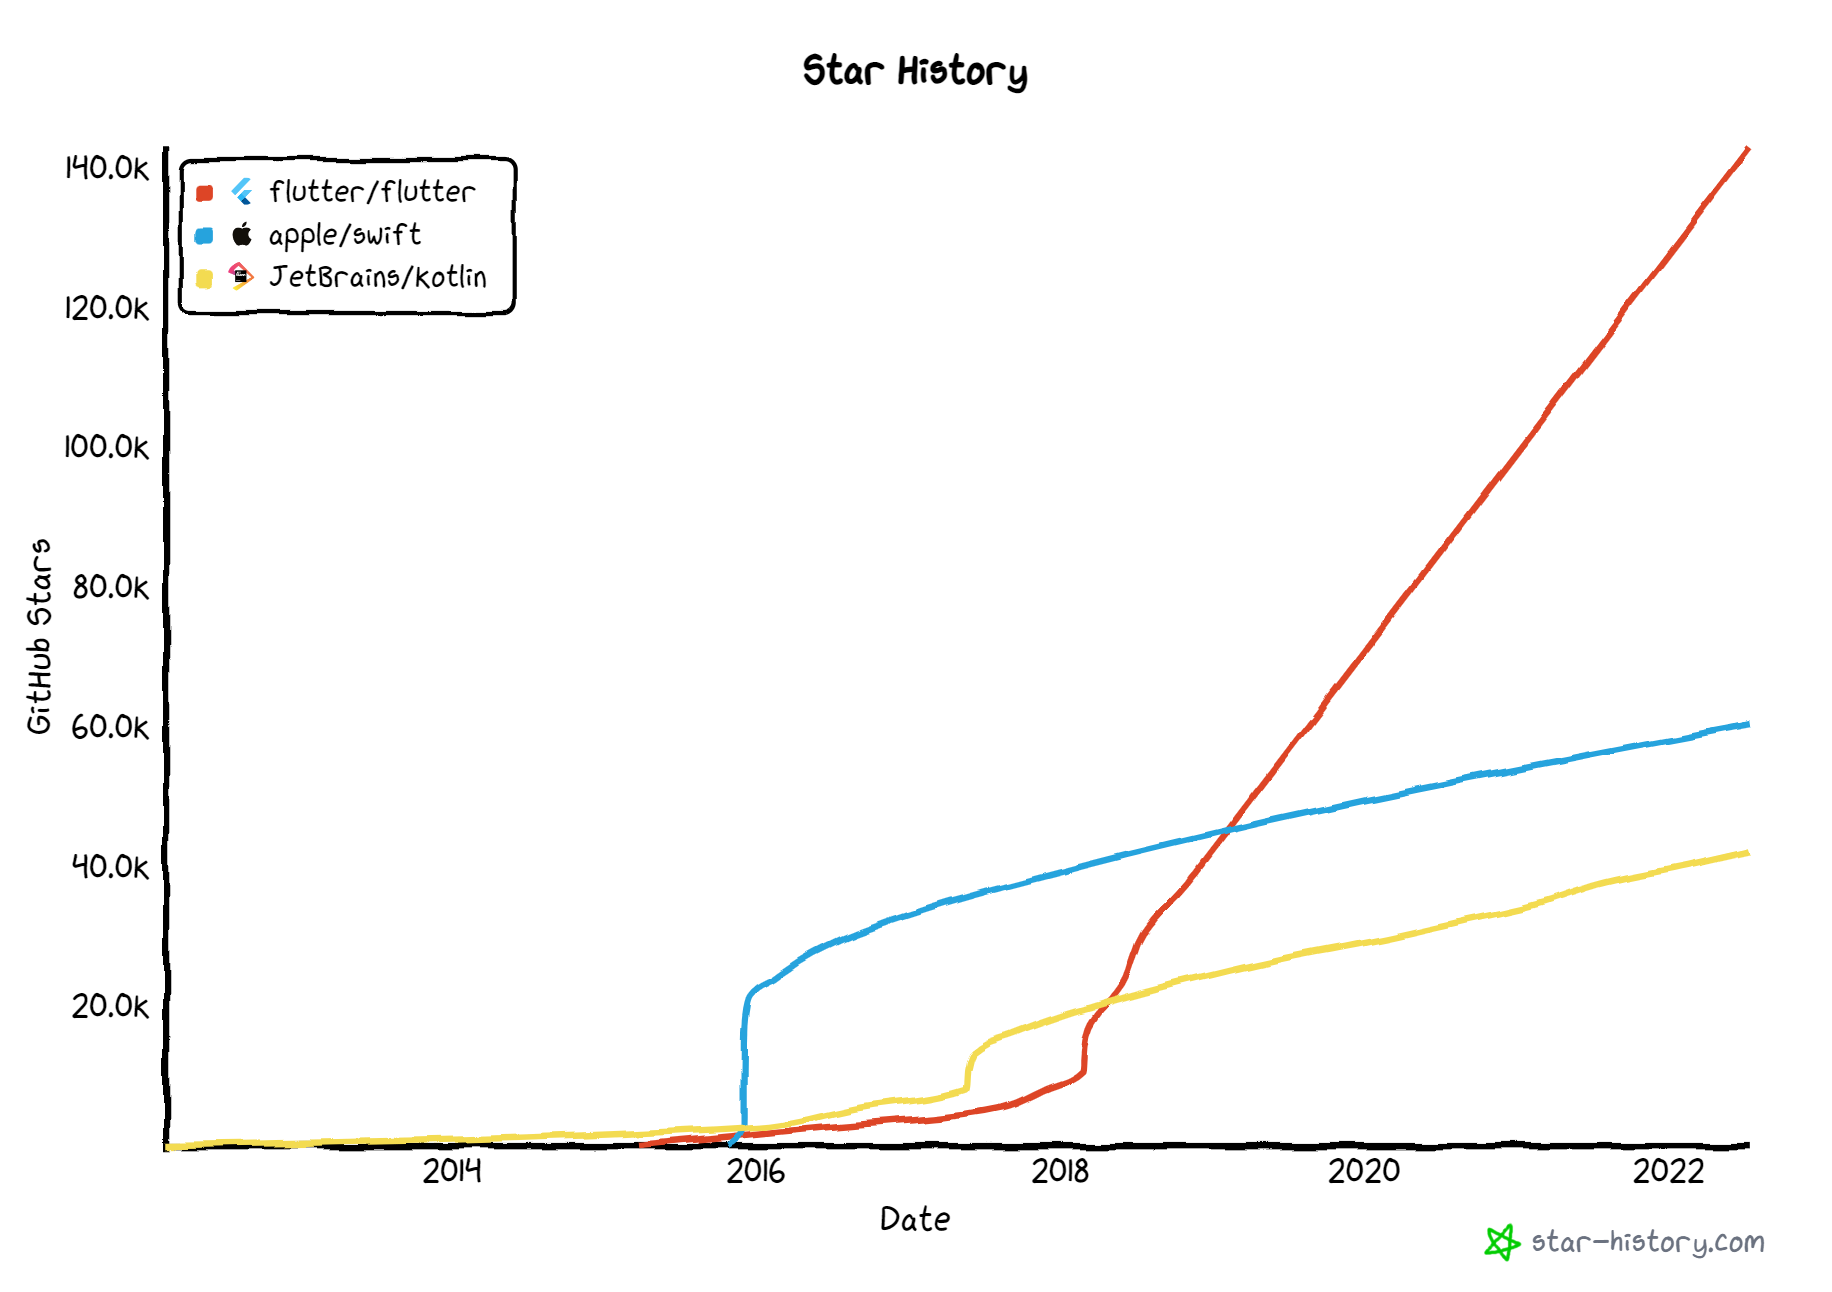
\includegraphics[height=7cm,keepaspectratio]{images/star-history_programming languages.png} 
  \caption[Zeitlicher Verlauf von Stars der Github-Repositorys von Swift, Kotlin und Flutter]{Zeitlicher Verlauf von Stars der Github-Repositorys von Swift, Kotlin und Flutter\protect\footnotemark }
  \label{fig:star_history}
\end{figure}
\footnotetext{https://star-history.com/\#flutter/flutter\&JetBrains/kotlin\&apple/swift\&Date}


Abbildung \ref{fig:star_history} zeigt ein mit Hilfe der GitHub-Api erstelltes Diagramm der Anzahl der Stars der Swift, Kotlin und Flutter Repositories im zeitlichen Verlauf. 
Besonders gut zu erkennen ist, wie stark das Interesse an Flutter ist. Nach der ersten Änkündigung 2018 und der darauf ersten veröffentlichten Version ist die Zahl der Interessierten innerhalb von 4 Jahren auf 140 000 angestiegen. Das Repository für Swift und Kotlin haben im gleichen Zeitraum gerade mal 20 000 Stars dazu erhalten. Dabei haben Swift und Flutter beide innerhalb des ersten Jahres nach Vorstellung etwa 30 000 Stars gemacht. Jedoch ist das Interesse an Swift danach abgeflacht und verläuft aktuell parallel zu Kotlin. Die Grafik zeigt, dass das Interesse an Flutter hoch ist, jedoch auch Kotlin und Swift Aufmerksamkeit erhält.

\subsubsection{Stackoverflow}
Ein weiterer Anhaltspunkt ist die Anzahl an gestellten Fragen auf Stackoverflow\footnote{https://stackoverflow.com/}. Stackoverflow ist für viele Entwickler ein guter Ort für Erklärungen oder Code, um die während der Entwicklung aufgetretenen Probleme zu lösen. Stackoverflow kann angemeldeten Nutzern, durch Filterung, die Anzahl der gestellten Fragen für einen Suchbegriff ausgeben. Hierfür wurde die Anzahl der Fragen für Kotlin, Swift und Flutter der letzten 2 Jahre gesammelt. Dabei wurden eventuelle Überschneidungen und Fragen ohne Antwort heraus gefiltert.

\begin{table}
\centering
\caption{Anzahl gefundener Fragen pro Programmiersprache}
\begin{tabular}{ |p{3.7cm}||p{5cm}| p{5cm}|}
 \hline
 Programmiersprache & Anzahl gefundener Fragen der letzten 2 Jahre & insgesamt gefundene Fragen\\
 \hline
 Kotlin &  105 082\footnote{Filter: [kotlin] or [android][kotlin] or [android]-[flutter]-[java] lastactive:2y.. is:question answers:1..} & 920 585\\
  \hline
 Swift  & 71 749\footnote{Filter: [swift] or [ios][swift] or [ios]-[flutter]-[objectivc] lastactive:2y.. is:question answers:1..} & 670 697\\
  \hline
 Flutter & 77,568\footnote{Filter:[flutter] or [dart] -[ubuntu] lastactive:2y.. is:question answers:1..} & 115 533\\
 \hline
\end{tabular}
\label{tab:evaluations_questions_stackoverflow}
\end{table}

Tabelle \ref{tab:evaluations_questions_stackoverflow} zeigt die ermittelten Werte. Flutter hat hierbei also eine ähnlich aktive Community, wie Kotlin und Apple. Hier muss jedoch eingeschränkt werden, dass manche Fragen schon vor dem untersuchten Zeitraum gestellt wurden und deswegen eine Frage nicht in dem untersuchten Zeitraum erneut auftaucht. So ist die Anzahl der insgesammt gefundenen Fragen mit mindestens einer Antwort sowohl bei Kotlin als auch Swift deutlich höher. Jedoch gibt es diese auch bereits eine längere Zeit. So zeigt sich, dass es sowohl für Kotlin als auch Swift genügend Fragen und Antworten gibt, um eine hohe Entwicklerzahl beziehungsweise vielen Hilfestellungen zu vermuten. Jedoch zeigt sich bei Flutter, dass es bereits in den letzten zwei Jahren mit den anderen beiden mithalten konnte und somit die Community stark am wachsen ist.

\subsubsection{Dokumentation}
Ein weiterer Faktor ist Dokumentation. Hierbei, haben sowohl Flutter als auch Kotlin und Swift eine umfangreiche und von den Entwicklern dauerhaft aktualisierte und erweiterte Dokumentationsseite. Wo jedoch Flutter einen Vorteil zu Kotlin hat, ist ein zentraler Ort\footnote{https://pub.dev/}, um nach weiteren Plugins, Bibliotheken, Widgets und vielem mehr zu suchen. Hier sind neben offizielle Flutter Repositorys, auch von der Community entwickelte Plugins verlinkt. In der Summe können hier bereits über 27000 Erweiterungen gefunden werden\footnote{https://pub.dev/packages?q=}. Neben einem Punktesystem, dass diese danach bewertet, wie viele Richtlinien eingehalten werden, wird außerdem angezeigt, welche Plattformen unterstützt werden. Zwar gibt es auch Ansätze bei Kotlin ein solches Verzeichnis einzuführen, jedoch sind diese nicht offiziell von der Entwicklerfirma betrieben und oft auch nicht vollständig. So muss teilweise nach GitHub-Repositories gesucht werden, um eine passende Bibliothek zu finden.

Neben der Dokumentation für die Programmiersprache kann man außerdem noch eine Programmierung für die verschiedene Entwicklungsansätze ziehen. Dabei hatten sowohl der cross-kompilierte, als auch der native Ansatz eine umfangreiche Dokumentation verfügbar. Für den gewählten hybriden Ansatz konnte Anhand von Anleitungen und Dokumentation der Programmiersprache eine ausreichende Unterstützung finden. Lediglich der gemischte Ansatz hatte hier Probleme. So konnte zwar gute Dokumentation für die gewählte Grundlagen und die Web Implementierung genutzt werden, jedoch ist eine Dokumentation für den genauen Ansatz nur begrenzt vorhanden. Dies liegt jedoch auch an der Art der Implementierung, da viele verschiedene Gemischte Implementierungen möglich sind und diese eher einen experimentellen Charakter besitzen.

Wie also erklärt wurde, gibt es sowohl für die hybride als auch die cross-kompilierte Implementierung eine vollumfängliche Dokumentation. Auch für den hybriden Ansatz lassen sich genügend Materialien finden. Dies dürfte sich bei der Nutzung eines Frameworks sogar noch verbessern. Lediglich der gemischte Ansatz hatte lediglich Grundlagendokumentation, jedoch keine für die Schwierigkeiten des Zusammenspiels. 

\subsubsection{Entwickler}
Ein letzter Faktor der zu dieser Kategorie analysiert werden soll, ist der Blick auf verfügbare Entwickler. Denn die Entwicklung einer Applikation in speziellen Technologien funktioniert nur, wenn auch Entwickler gefunden werden können. Eine Statistik \cite{statist_used_programming_languages} der Firma Stackoverflow besagt, dass etwa 9\% Kotlin, 7\% Dart und 5\% Swift der 71,547 befragten Entwicklern beherrschen.
Bei den Programmiersprachen für Web, gaben  65\% an, JavaScript zu kennen und 55\% kennen sich in HTML bzw. CSS aus. Diese Zahlen lassen den Schluss zu, dass die Ansätze mit einem hohen Anteil an Web Technologie einen Vorteil haben, da es einfacher sein dürfte, passende Entwickler zu finden. Jedoch wird auch bei den Ansätzen mit Webtechnologie mindestens ein Entwickler benötigt, der sich mit den einzelnen Plattformen genauer auskennt, falls es Schwierigkeiten gibt, oder Plattform spezifische Funktionalität selber erstellt werden soll.

Zusammenfassend lässt sich sagen, dass es für alle Ansätze genügend Entwickler geben wird, jedoch haben die hybriden und die Flutter-Web Implementierung dahingegen einen Vorteil, dass ein wesentlicher Teil aus einer Webseite oder Webtechnologie besteht und es hier eine deutlich höhere Anzahl an Entwicklern gibt.

\section{Entwicklungsdauer}
Ein weiteres wichtiges Kriterium bei der Wahl des Ansatzes ist die Entwicklungsdauer, da diese sich auf die Kosten der entwickelten Multi-Plattform-Anwendung auswirkt. Daher soll diese im Folgenden anhand zweier Faktoren etwas beleuchtet werden.

\subsubsection{Programmieraufwand}
Die genaue Entwicklungsdauer ist stark von der Erfahrung der Entwickler und eventuell auftretenden Problemen während derImplementierung abhängig, weswegen ein Zeitvergleich hier nicht sinnvoll erscheint. Stattdessen soll die Anzahl der geschriebenen Programmzeilen (LOC) betrachtet werden.
Dafür wurden die einzelnen Daten mit Hilfe des Statistics\footnote{https://plugins.jetbrains.com/plugin/4509-statistic} Plug-In von JetBrains gesammelt.
Bei den beiden Implementierungen mit Web-Anteil wurde außerdem der notwendig Teil der Web-Implementierung mit angegeben. 
Dabei wurden die gesammelten Daten in die drei Arten aufgeteilt: Konfiguration, Benutzeroberfläche und Logik unterteilt. 
Bei den Implementierungen, bei denen Flutter genutzt wurde, ist der UI- und Logikcode zusammengefasst, da dies bei Flutter in einer Datei geschrieben wird.
Als weiterer Parameter wurde der benötigte Code untersucht, um eine Liste an Gegenständen anzuzeigen.
Dabei wurden nur tatsächlich geschriebene Code-Teile betrachtet und automatisch generierte nicht gezählt.


\begin{table}
\centering
\caption[Programmlänge der verschiedenen Implementierungen in LOC]{Programmlänge der verschiedenen Implementierungen in LOC}
\begin{tabular}{ |p{4.5cm}||p{3cm}|p{2cm}|p{2cm}|p{3cm}|p{3cm}| }
 \hline
 Programmteile in Lines of Code & Flutter-Web & Flutter & Kotlin-Nativ & Kotlin-Hybrid \\
 \hline
 Gesamte Anwendung       &   2391(App) + 1533(Web) &   2100 & 3138 & 215(App) + 2814(Web)\\
  \hline
 Konfigurationscode  & 42 + 268& 32& 229& 30 + 357\\
  \hline
 Oberflächencode &\multirow{2}{*}{2349 + 1265}  &\multirow{2}{*}{2068}  & 1958& 86 + 1768\\
  \cline{1-1}
  \cline{4 -5}
 Funktionalität \& Logik & & & 951& 99 + 689\\
  \hline
 Beispiel: Liste an Gegenständen & 65(App) & 65 & 178 & 71(Web)\\
  \hline
\end{tabular}
\label{tab:lines_of_code}
\end{table}

Die in Tabelle \ref{tab:lines_of_code} zu sehende Aufschlüsselung zeigt, dass Flutter insgesamt die wenigsten Zeilen an Code benötigte. 
Dabei werden gerade einmal 32 Zeilen Code Konfiguration benötigt. 
Der Rest sind knapp 2000 Zeilen Code mit Benutzeroberfläche und Logik. Die native Implementierung benötigt diese Anzahl allein um die Benutzeroberfläche zu definieren und benötigt knapp 1000 weitere Zeilen um die Funktionalität und Logik hinzuzufügen. 
Den höchsten Programmieraufwand benötigt der gemischte Ansatz. Er kommt insgesamt auf knapp 4000 Zeilen Code und damit den doppelten der Flutter Implementierung. Die native und die hybride Implementierung haben in etwa die gleiche Anzahl an Zeilen Code und liegen mit rund 3000 Zeilen Code in der Mitte zwischen den zwei anderen Implementierungen.
In der implementierten Anwendung hat die native Implementierung mit gerade einmal 215 Zeilen Code den geringsten Umfang, jedoch kommen hier rund 2800 Zeilen Web-Implementierung dazu.

Bei dem zusätzlich betrachteten Beispiel, einer dynamischen Liste für Gegenstände ohne fester Länge, ist die Flutter Implementierung ebenfalls die kürzeste. Dabei werden gerade einmal 65 Zeilen Code benötigt, wovon 55 Zeilen auf die Anzeige eines Gegenstandes und gerade einmal 10 Zeilen Code auf die Liste entfallen. Ähnlich ist dies bei der Webseite. Einzig die native Kotlin Applikation hat hier ein erhöhten Aufwand. Dabei entfallen 75 Zeilen auf das Design und weitere 83 Zeilen auf die Steuerung der Liste und dem hinzufügen der Daten. Ein Großteil davon ist der Adapter, der benötigt wird um die Liste zu steuern. Die Web-Implementierung der hybriden Applikation braucht mit 71 Zeilen, ähnlich wenige wie die zwei Flutter-Implementierungen.

Ein weiterer Faktor der beachtet werden muss, ist die Anzahl der nötigen Implementierung je Ansatz. So ist bei dem gemischten und dem cross-kompilierten Ansatz lediglich eine Implementierung nötig. Beim nativen Ansatz muss jedoch je unterstützter Plattform eine eigenständige Implementierung erstellt werden. Bei der hybriden Applikation, wie sie in dieser Arbeit umgesetzt wurde, ist zwar die umgebende Applikation ebenfalls für jede Plattform zu implementieren, jedoch hat die Implementierung einen deutlich geringeren Umfang. Der Teil der Web-Anwendung muss lediglich einmal geschireben werden.  

Wie also gesehen werden konnte, benötigt eine cross-kompilierte Lösung mit Flutter deutlich weniger Zeilen Code als die anderen Implementierung.
Wenn jedoch bereits eine Web-Anwendung existiert, reduziert sich der Implementierungsaufwand der hybriden Aufwand auf knapp 200 Zeilen Code und der gemischten Implementierung halbiert sich in etwa. Dadurch können diese beiden Implementierungen in dieser Situatuin ebenfalls eine gute Alternative zu den anderen Ansätzen darstellen. Muss diese jedoch erst erstellt werden ist gerade der gemischte Ansatz mit einem erhöhten Aufwand verbunden.

\subsubsection{Zeit bis zur Veröffentlichung}
Die Entwicklungsdauer wirkt sich direkt auf auch auf den Faktor der Dauer bis zur Möglichkeit der Veröffentlichung einer ersten Version aus .
Je früher eine Anwendung veröffentlicht werden kann, desto früher können Kunden die Applikation nutzen und bei einer kommerziellen Nutzung auch Umsatz produzieren.

Hierbei ist sowohl die native und die cross-kompilierte Implementierung auf eine vollständige Implementierung angewiesen, um den Nutzer ein umfängliches System zu bieten. Bei der nativen Entwicklung kommt d
Durch den Programmieraufwand und der Anzahl der zu unterstützenden Plattformen wird die Dauer der Entwicklungszeit und die Zeit bis zu einem möglichen Release stark beeinflusst. Genaue Werte sind dabei auch stark von Funktionsumfang, Anzahl der Entwickler und den Vorraussetzungen abhängig. Jedoch lassen sich dennoch einige Aussagen treffen.

So ist etwa ein Release der Nativen Anwendung am aufwendigsten. Nicht nur dass wie bereits gesehen, mit der meiste Code geschrieben werden muss, muss dies auch noch für jede Plattform passieren. Am schnellsten ist dies bei der Cross-Plattform Implementierung mit Flutter. Hier muss lediglich einmal die Anwendung durchprogrammiert werden und kann im Anschluss für die einzelnen Plattformen einfach nur noch exportiert werden. Nach der reinen Flutter Implementierung ist die Flutter Implementierung mit Webanteil. Diese ist dann gefolgt vom hybriden Ansatz. 

Wenn jedoch die Webseite bereits existiert und dementsprechend nicht bei der Implementierzeit beachtet werden muss, ändert sich hier die Reihenfolge sehr wahscheinlich je nach umfänglichkeit der Zusatz Implementierung des Flutter Web Ansatzes.

Der Flutter-Web Mixansatz kann außerdem noch von hohem Vorteil sein, wenn eine Webseite in eine App verwandelt werden soll. Denn hier kann wie bei der hybriden Implementierung eine anfängliche Version veröffentlicht werden, die lediglich die Webseite öffnet und danach Stück für Stück die Webseite durch Flutter Seiten ersetzen. So kann der Nutzer jederzeit die komplette Anwendung nutzen und bekommt Stück für Stück eine angepasste Appversion.

\section{Nutzeroberfläche}
\subsubsection{Aussehen der Applikationen}
Grundsätzlich ist das Aussehen der Applikation vor allem davon abhängig, wie viel Zeit hierfür investiert wird. Jedoch können anhand der Applikationen dennoch einige Beobachtungen angestellt werden.

\begin{figure}[ht]
  \centering
  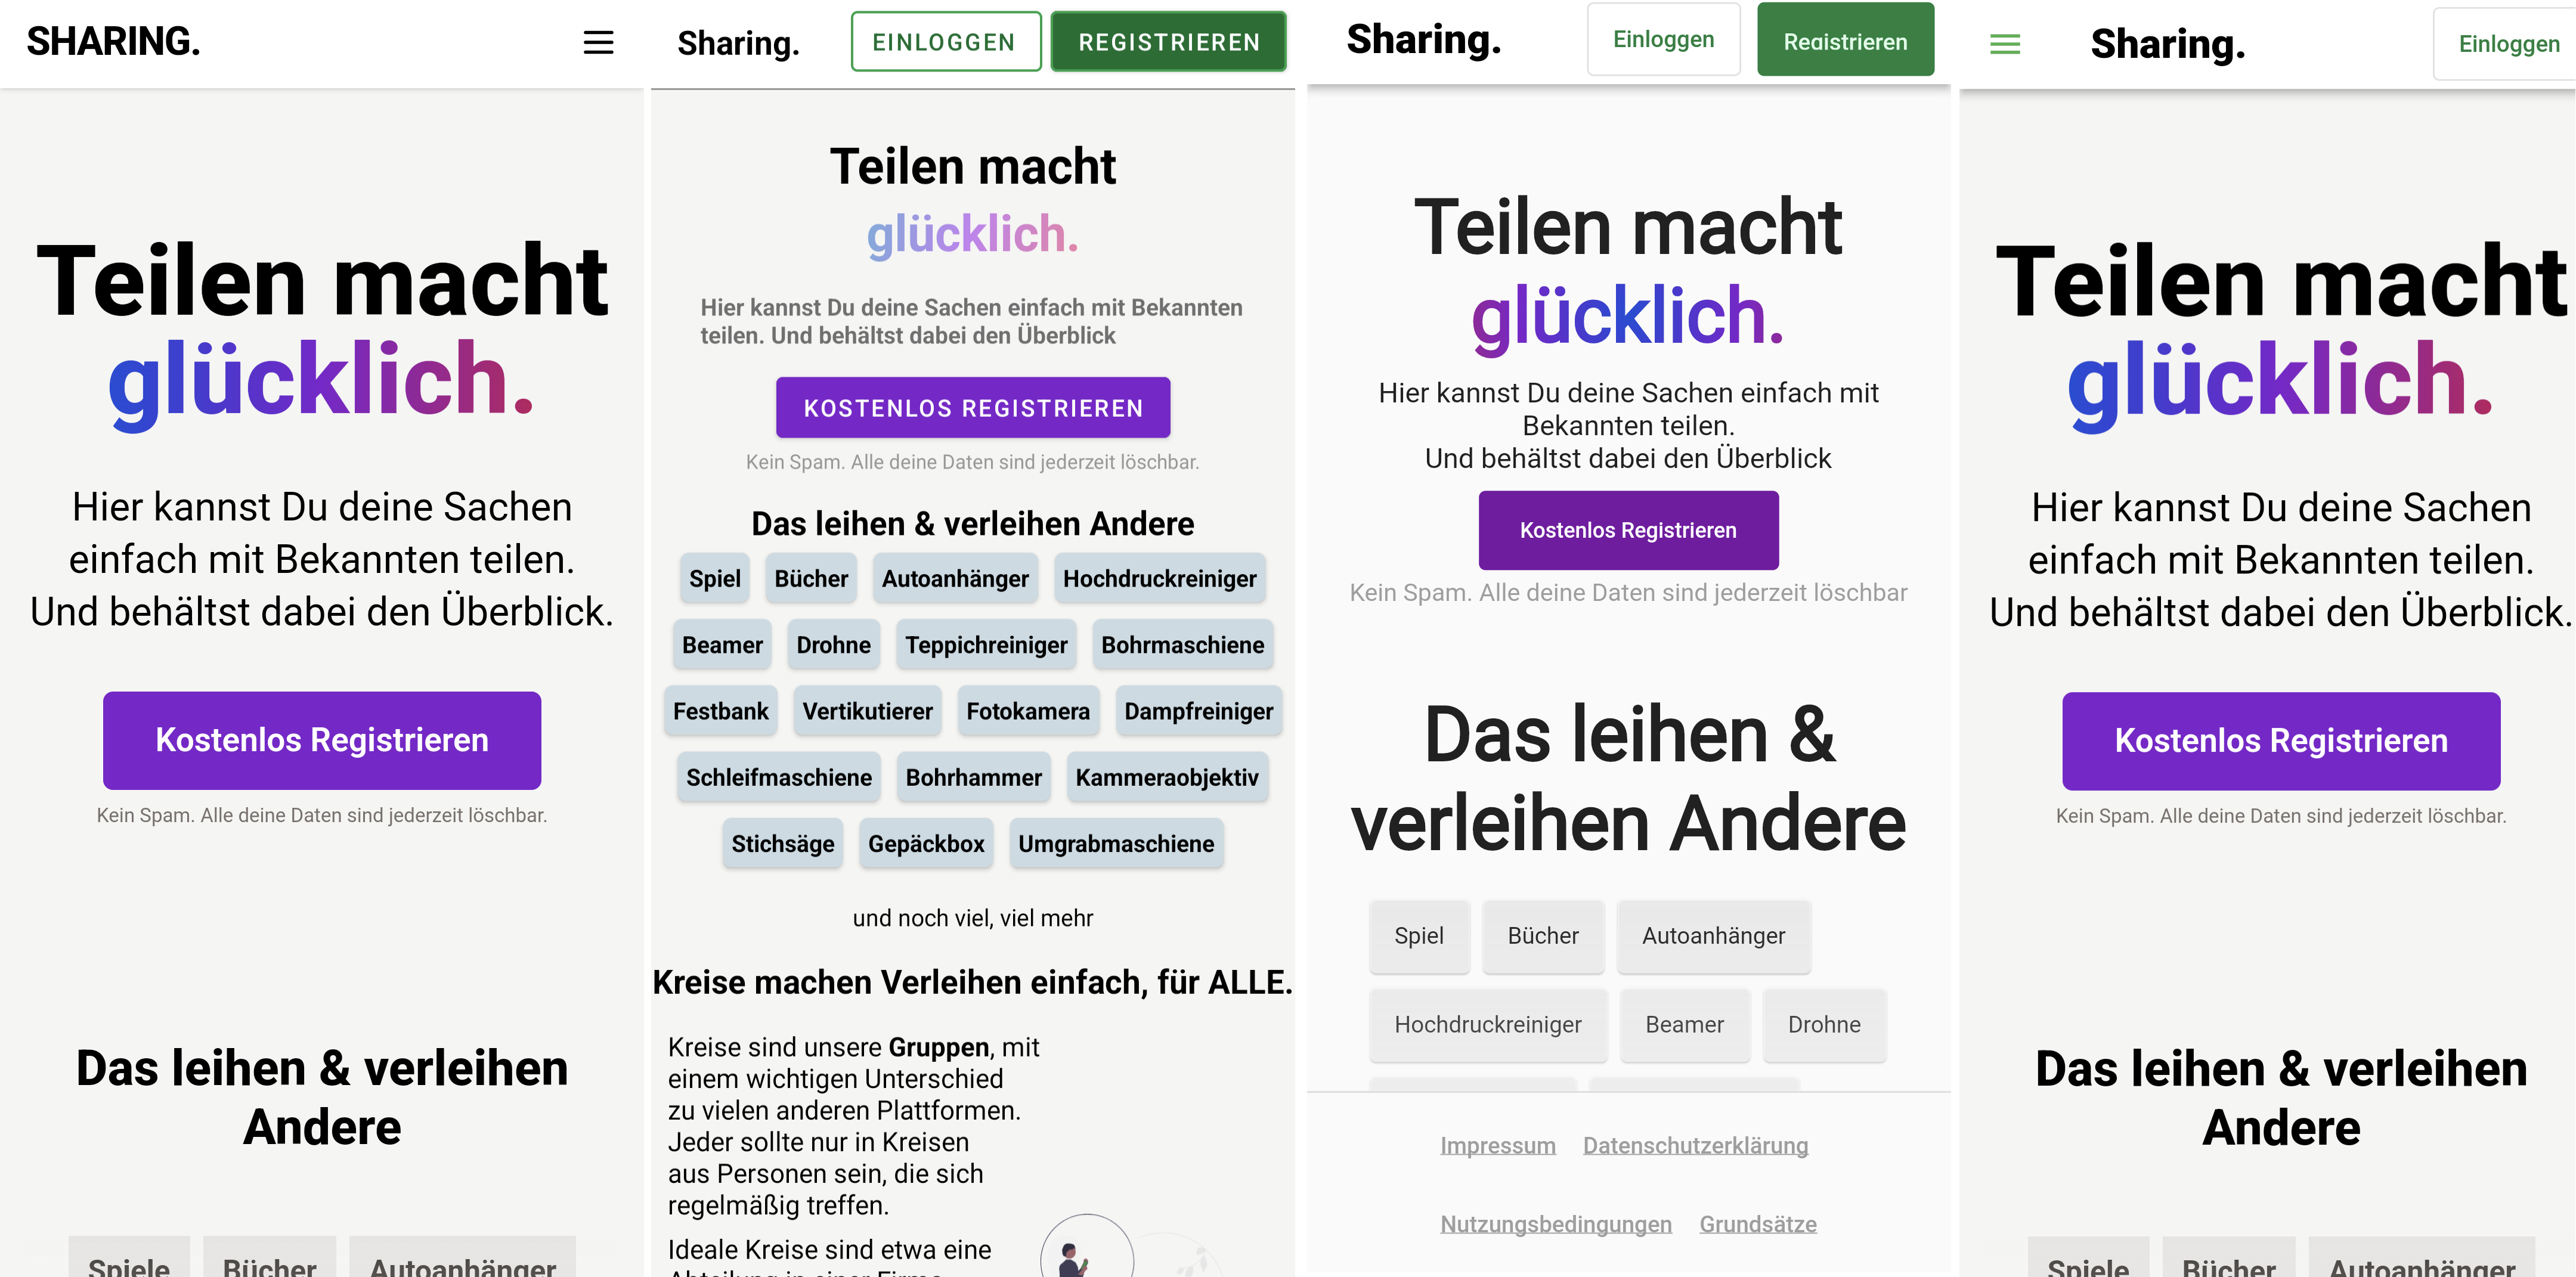
\includegraphics[height=7cm,keepaspectratio]{images/Startbildschirm_vergleich.png} 
  \caption[Vergleich des Startbildschirms der Implementierungen]{Vergleich des Startbildschirms der Implementierungen. Von links nach rechts: Hybride-Applikation, native Kotlin Applikation, Flutter Cross-Plattform-Applikation, Flutter Hybride Applikation}
  \label{fig:startscreen}
\end{figure}

In Abbildung \ref{fig:startscreen} sind die Startbildschirme der verschiedenen Anwendungen zu sehen. Für alle wurde eine etwa gleich lange Maximalzeit verwendet, um das Ergebnis vergleichen zu können. Der erste Bildschirm ist von der Webversion. Für diese wurde am wenigsten Zeit genutzt, da an ihr nicht viel geändert werden konnte. Sie ist also die gleiche Darstellung wie wenn die Webseite im Browser aufgerufen werden würde.  Sie ist, wie es auffällt bereits stark für mobile Geräte optimiert und sieht dementsprechend gut nutzbar aus. Was bei ihrer jedoch negativ auffällt, sind die nicht nativen Elemente durch die reine Nutzung von JavaScript.
So ist in Abbildung \ref{fig:sidemenu} die Seitenmenüanzeigen anhand von Flutter und durch die Webimplementierung gezeigt. Hier merkt man bei der Nutzung deutlich, dass die Web-Implementierung für PC Nutzer ausgelegt ist, mit dem Ziel gut für Smartphone Nutzer bedient zu werden, während die Flutter Implementierung deutlich besser für die Nutzung an einem Smartphone ausgelegt ist. Dies ist besonders gut spürbar, da das Menü der Webseite nur über einen Knopf und manuelles drücken nutzbar ist, während in der Flutter Implementierung von der Seite gewischt werden kann um die Vorteile eines Touchscreens auszunutzen.

\begin{figure}[ht]
  \centering
  \includegraphics[height=7cm,keepaspectratio]{images/Seitenmenü_vergleich.png} 
  \caption[Vergleich des Seitenmenüs der nativen und hybriden Applikation]{Vergleich des Seitenmenüs bei nativer Implementierung (links) und JavaScript Implementierung (rechts).}
  \label{fig:sidemenu}
\end{figure}

Während auf der Webseite einiges an Zeit und ein extra Designpakete genutzt wurden, um das insgesamte Aussehen der Anwendung zu verändern, wurde bei den getroffenen Implementierungen lediglich die Farben angepasst. Bei der Flutter Implementierung wirken die Elemente dabei deutlich moderner und angepasst für eine Smartphone-Applikation. Das wird besonders deutlich, wenn die Login-Screens verglichen werden.

\begin{figure}[ht]
  \centering
  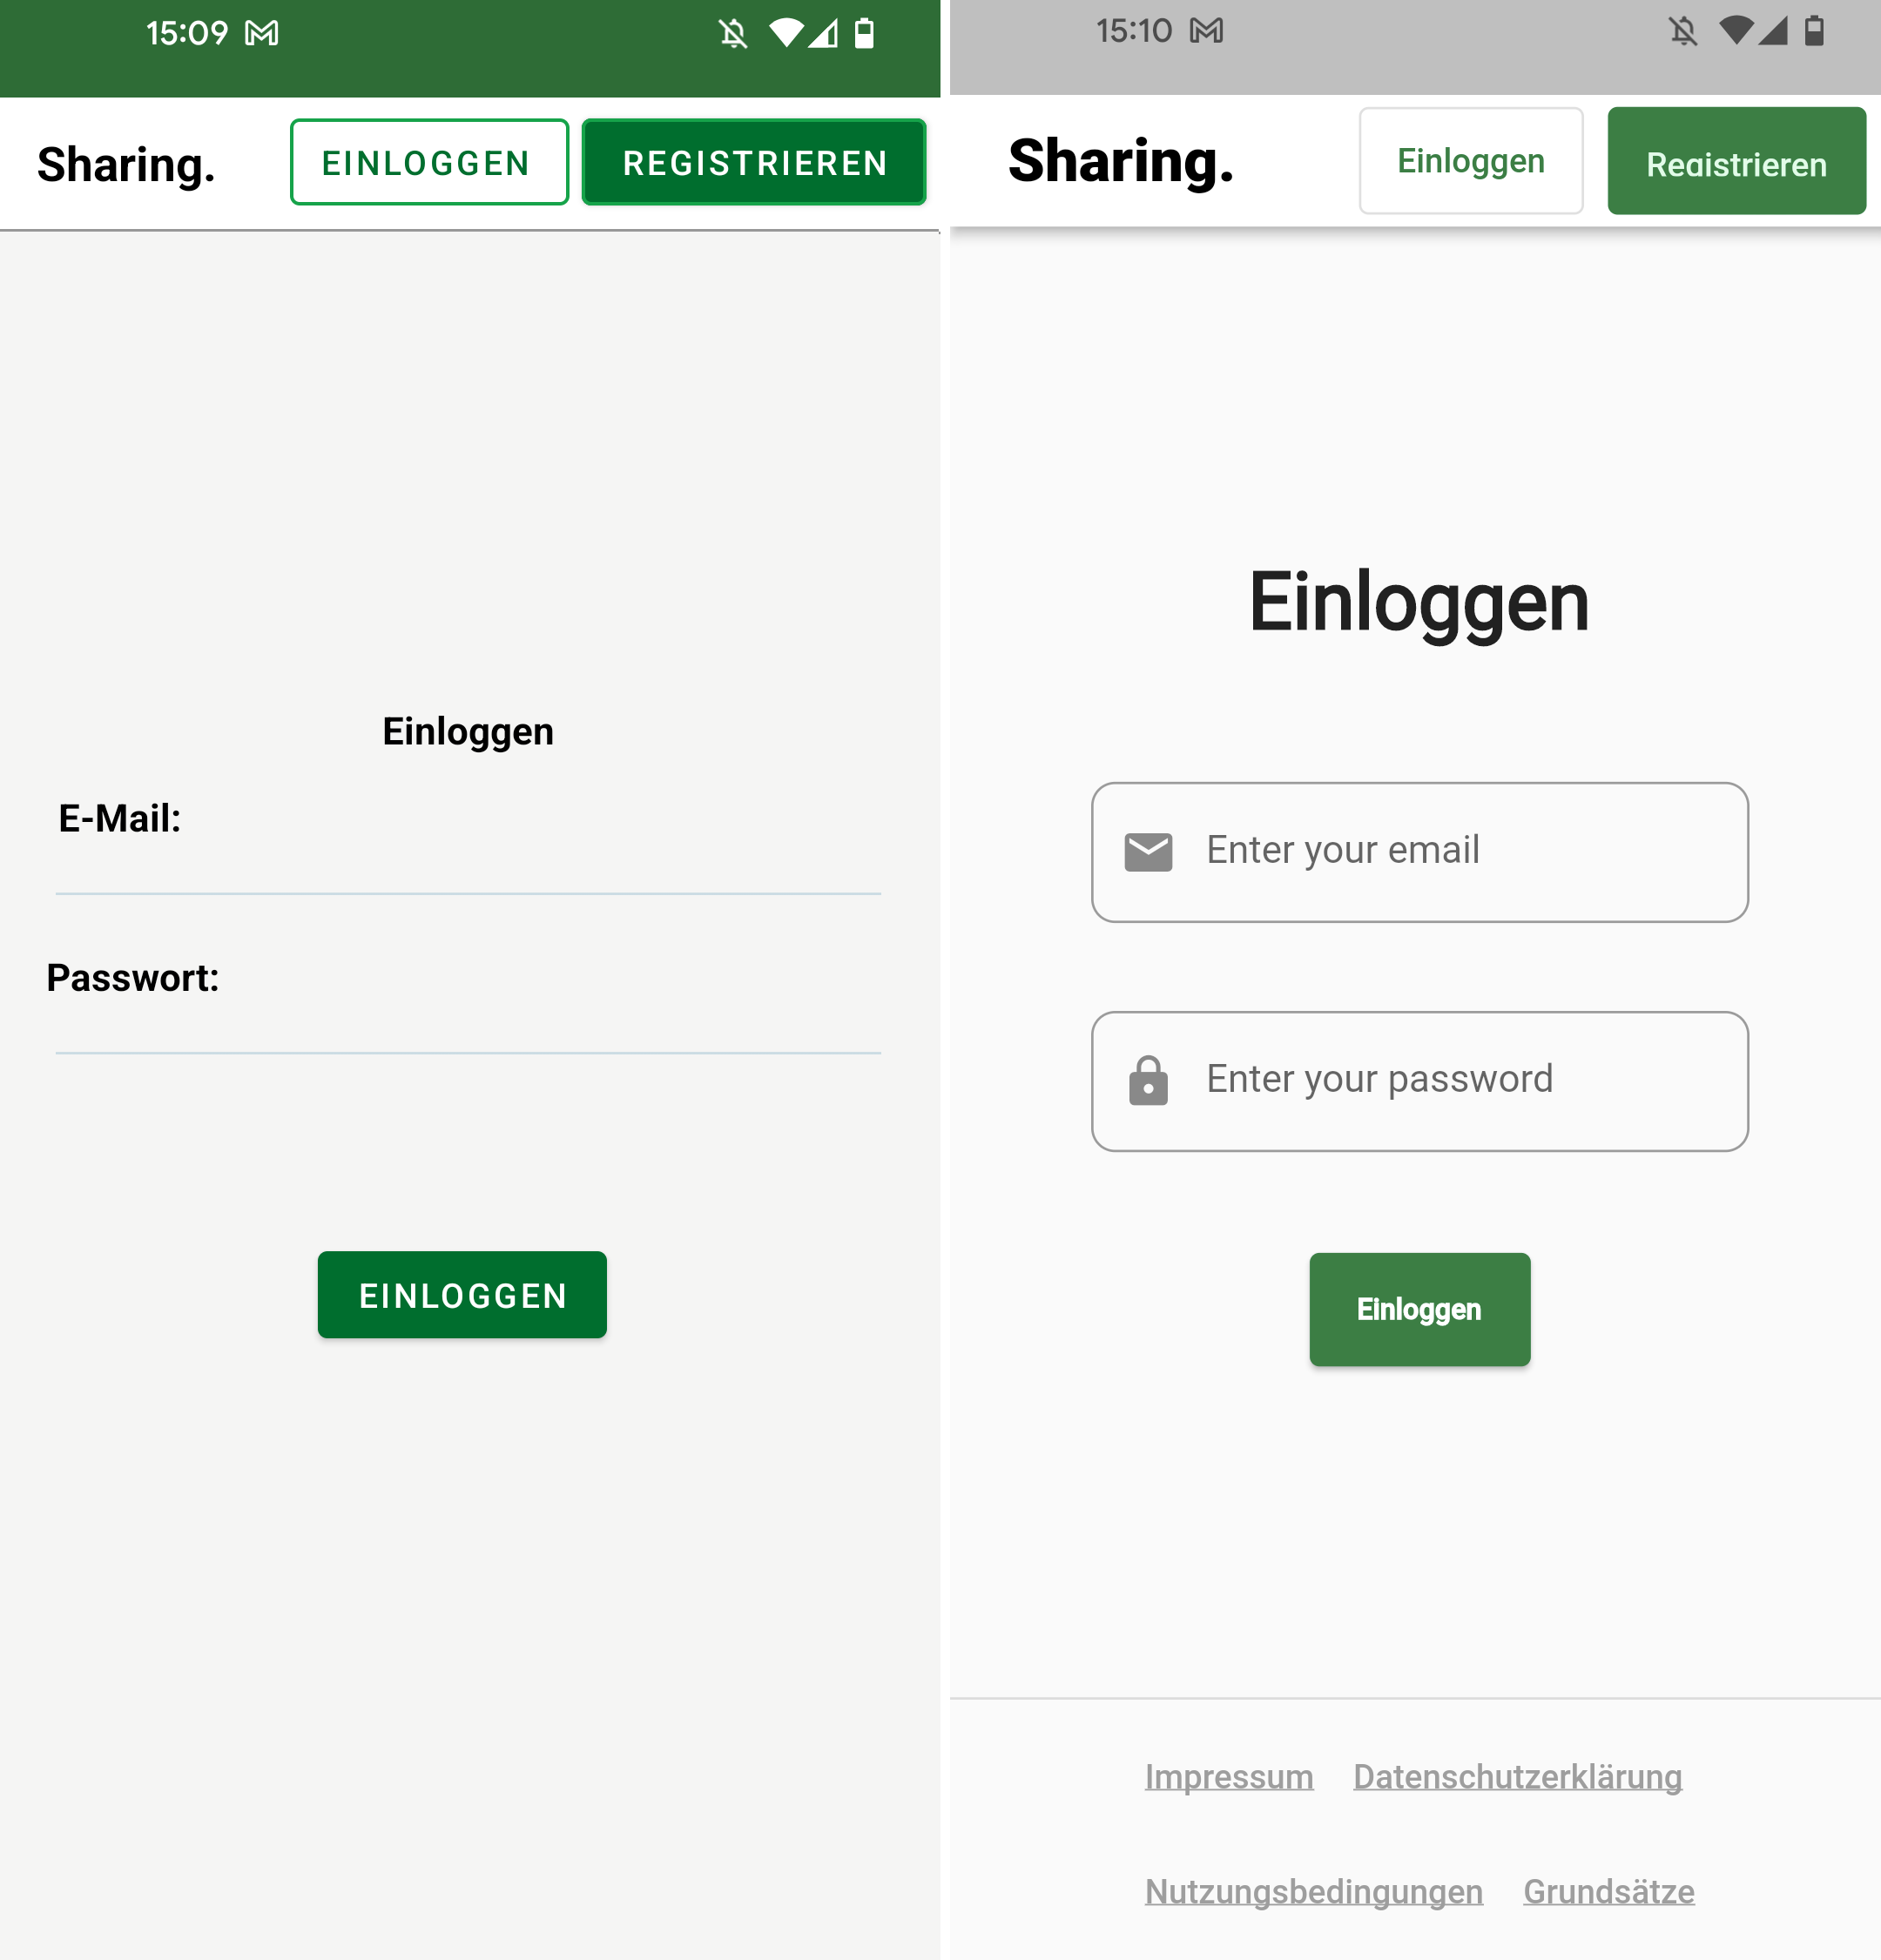
\includegraphics[height=7cm,keepaspectratio]{images/Login_vergleich.png} 
  \caption[Vergleich des Login-Bildschirms von Kotlin und Flutter Implementierung.]{Vergleich des Login-Bildschirms von Kotlin (links) und Flutter (rechts) Implementierung.}
  \label{fig:loginscreen}
\end{figure}

In Abbildung \ref{fig:loginscreen} ist der Loginscreen der nativen und des Cross-compilierten Ansatzes zu sehen. Hier wurde bis auf Farbanpassungen keine größeren Anpassungen vorgenommen, um einen Eindruck für das Standardaussehen der einzelnen Komponenten zu erhalten. Wie bereits erwähnt hat Flutter ein deutlich besseres Out-of-the-Box Design Paket. Die Input Felder bei der Koltin Implementierung wirken dabei recht unscheinbar und unauffällig, so dass diese für ein fertiges Produkt noch einmal angepasst werden müssten, um Nutzerfreundlich zu sein.

Das Aussehen der einzelnen Apps ist aber durch Erweiterungen und sonstigen stark anpassbar, sodass mit genügend Zeit und Wille alle Applikationen egal mit welchen Ansatz sehr ähnlich aussehen könnten. Wie aber ersichtlich geworden ist, bietet Flutter die am modernsten und passend wirkende Standardkonfigutration für die Benutzeroberflächen. So ist die Entwicklung einer UI in Flutter deutlich schneller und mit weniger Konfigurationsaufwand verbunden, als mit jeder anderen betrachteten Implementierung.

\subsubsection{Konsistenz über Plattformen hinweg}
Ein weiterer Aspekt bei der Entwicklung der Nutzeroberfläche ist die Konsistenz über Plattformen hinweg. Das Ziel ist es dabei, dass der Nutzer keinen Unterschied bemerkt, wenn er von einer Plattform zu einer anderen wechselt. 
Dies bedeutet, dass wo immer unterschiedliche Implementierungen für die Plattformen geschrieben werden, die Gefahr für Inkonsistenz am höchsten ist.
Dementsprechend sind Implementierungen die für mehrere Plattformen wieder verwendet werden können ein positiver Faktor um die Konsistenz zu fördern.
Auf die in dieser Arbeit vorgestellten Implementierungen bezogen, bedeutet dies, dass die reine native Implementierung eine höhere Gefahr von Inkonsistenz besitzt, als etwa die hybride oder Flutter Applikation.
Dabei ist allerdings zu erwähnen, dass auch die nativen Applikationen einen hohen Grad an Konsistenz erreichen können. Dies bedeutet jedoch häufig einen höheren Aufwand bei der Implementierung und eine enge Zusammenarbeit der Entwickler der verschiedenen Plattformen.

\section{Sonstiges - Funktionalität- noch nicht richtiger Titel}

\subsubsection{Plattformabdeckung \& Wiederverwendbarkeit}
Wie an mehreren Stellen der Arbeit bereits erwähnt sind nativ entwickelte Applikationen immer nur für eine Plattform entwickelt. Sie haben dementsprechend auch den am wenigsten wiederverwendbaren Code, da lediglich die Logik geteilt werden kann, jedoch die genaue Implementierung für jede Plattform unterschiedlich ist. Jedoch kann für jede Plattform eine native Apllikation geschrieben werden.

Hybride Apps haben hier bereits einen deutlich höheren Wiederverwenbarkeitsgrad, da bei ihnen ja lediglich die Anzeigelogik ausgetauscht werden muss, aber die iegentliche Implementierung in einer Webtechnologie getan wurde, wodurch sie auf fast jeden Gerät genutzt werden kann. Jedoch können einige Technologien auf ein paar Plattformen beschränkt sein. Desweiteren kann es bei dieser Klasse durchaus Probleme geben, wenn sie zu einem großen Anteil aus der Ansicht der Webseite besteht. So wurde ja bereits die Richtlinien von Apple erwähnt, die diese Klasse zu einem gewissen Grad aus dem App-Store verbannt. Da hybride Applikationen außerdem einen nativen Code-Teil besitzen, sind sie wieder nur auf einer Plattform installierbar. 

Cross-Plattform-Applikationen werden mit einer Technologie gebaut, um mehr als eine Plattform mit einem Code abzudecken. Dabei ist dies zwar von der genau genutzten Technologie abhängig, aber in dem vorgestellten Fall sind 5 Plattformen damit abdeckbar. Mit Flutter und der Wahl der richtigen Erweiterungen sind nach aktuellem Stand sogar 6 Plattformen möglich. Außerdem kann durch die Wahl von Flutter der gleiche Code für alle Plattformen genutzt werden. Eine Wiederverwendbarkeit ist so gesehen also nicht bewertbar, da es theoretisch nicht nötig ist den Code für eine andere Implementierung wiederzuverwenden. Wenn allerdings der Code für eine andere Implementierung genutzt werden sollte ist es wie im nativen Fall, dass nur die Applikationslogik nutzbar ist, da die Anwendung in ihrer eigenen Programmiersprache geschrieben ist.\TODO{https://flutter.dev/multi-platform/embedded}

Die Flutter-Web Implementierung ist in diesem Aspekt ähnlich zu der Flutter Implementierung. So gelten grundsätzlich die gleichen Aussagen, jedoch mit Einschränkung der Anzahl der abgedeckten mobilen Endgeräte. So ist diese Implementierung lediglich auf den beiden Plattformen Android und iOS nutzbar. Wie bereits erwähnt ist dies Abhängig von der Web-Container Implementierung und kann mit der Wahl eines passenderen Containers oder Eigenentwicklung eines eigenen Browser-Plugins auf die restlichen Plattformen erweitert werden.

\subsubsection{Offline Funktionalität}
Es gibt einige Fälle in denen der Nutzer unter Umständen eine Applikation weiter nutzen will, auch wenn er aktuell keine aktive Internetverbindung hat. In diesem Fall benötigt die Applikation eine offline Funktionalität.

Wie bereits an mehreren Stellen in dieser Arbeit erwähnt haben die Implementierungen, die die Webseite als Teil ihrer Implementierung haben, hier oft keine Funktionalität. Im Falle der Flutter-Web Applikation kann die Funktionalität zumindest teilweise erreicht werden, indem andere Seiten angezeigt werden die nativ implementiert werden. Die native und Cross-Compilierte Lösung haben hier eindeutig den besseren Standpunkt. Ihre Anzeige ist unabhängig von einer aktiven Internetverbindung nutzbar. Hier kommt es lediglich darauf an, ob die Daten, die in der App angezeigt werden auf dem Gerät gespeichert werden oder ob sie immer von einem Server abgefragt werden müssen. 

Hier ist allerdings zu erwähnen, dass andere hybride Ansätze zwar auch Webtechnologie nutzen, jedoch die Daten alle lokal auf dem Gerät gespeichert werden. In diesem Fall hätte auch der hybride Ansatz offline funktionieren. Der in diese Arbeit gewählte Ansatz jedoch nicht.

\subsubsection{Nutzung von Plattformfunktionalität}
Sowohl die nativen als auch die Cross-Compilierte Lösung mit Flutter hat die Möglichkeit, mit der richtigen Programmierung, alle Funktionalitäten der Hardware zu nutzen.
\TODO{Quellen}
Die hybriden und Web-Applikationen haben hierbei den Nachteil, dass Webseiten nur auf die Funtkionalitäten unterstützt, den auch Browser unterstützen. Jedoch die hybriden Ansätze die zwar mit einer Webtechnologie funktionieren, aber auf dem Gerät lokal laufen können über Schnittstellen ebenfalls auf die Funktionalität zugreifen
\TODO{Vielleicht auch raus.}

Einen Vorteil den native Applikationen haben ist, dass alle verfügbare Funktionalität in die eigene Applikation eingebunden werden können, selbst wenn es sie auf anderen Plattformen nicht existiert.

Um dies zu erreichen, müsste bei Cross-Plattform Ansätzen eine Unterscheidung zwischen Plattformen stattfinden, wie dies etwa in Flutter mit Hilfe der Abfrage der TargetPlatform\footnote{https://api.flutter.dev/flutter/foundation/defaultTargetPlatform.html} geschehen kann. Die Frage ist dann jedoch wie sinnvoll dies ist, da dadurch Unterschiede zwischen den Plattformen entstehen, die bei den Cross-Platformen eben nicht entstehen sollen.
